\section{Ход работы, результаты}

\subsection{Установка}
\begin{figure}[H]
    \centering
    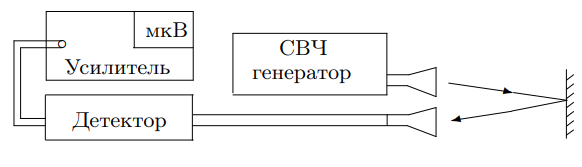
\includegraphics{pic/setup0.png}
    \caption{Схема приёмно-передающей системы СВЧ-диапазона}
    \label{fig:setup0}
\end{figure}
Для генерации и приёма волн СВЧ-диапазона использовалась установка, изображённая на рис. \ref{fig:setup0}. Применяемый в настоящей работе передатчик излучает линейно поляризованную волну с частотой $\nu\approx36$ ГГц, электрический вектор $\mathbf{E}$ которой направлен вертикально. Приёмник также может принимать только линейно поляризованную волну, причём в ходе опытов он работал в квадратичном режиме, поэтому получаенные на усилителе сигналы были пропорциональны интенсивности излучения. Для изменения угла отражения волны зеркало (металлическая пластинка) было установлено на вращающейся подставке.

Установка была настроена и отъюстирована, на вольтметре приемника был получен максимальный сигнал. Затем на пути СВЧ волн были помещены различные препятствия для исследования их проницаемости:
\begin{itemize}
    \item Бумажный лист незначительно ослабил сигнал.
    \item Диэлектрическая пластинка более значительно изменила сигнал, чем бумага, но не погасила совсем.
    \item Металлический лист полностью перекрыл волны, отразив и частично поглотив их.
\end{itemize}

\subsection{Проверка закона Малюса}
При изменении угла падения в пределах от 0$^\circ$ до 37$^\circ$ между выходным напряжением приемника и квадратом косинуса угла действительно наблюдалась примерно линейная зависимость, что позволяет утверждать о выполнимости закон Малюса и линейной поляризованности волн в эксперименте. Результаты измерений представлены в таблице \ref{tab1} и графике \ref{graph1}.

\begin{table}[!ht]
    \centering
    \begin{tabular}{|l|l|l|l|}
    \hline
        $\theta, ^\circ$ & $\cos \theta$ & $\cos^2 \theta$ & $I, \text{мкВ}$ \\ \hline
        37 & 0,800 & 0,64 & 0 \\ \hline
        32 & 0,849 & 0,72 & 8 \\ \hline
        27 & 0,892 & 0,80 & 20 \\ \hline
        22 & 0,927 & 0,86 & 36 \\ \hline
        17 & 0,957 & 0,92 & 46 \\ \hline
        12 & 0,977 & 0,96 & 59 \\ \hline
        7 & 0,992 & 0,99 & 68 \\ \hline
        0 & 1 & 1,00 & 76 \\ \hline
    \end{tabular}
    \caption{Зависимость интенсивности отражённого луча от угла падения}
    \label{tab1}
\end{table}

\begin{figure}[H]
    \centering
    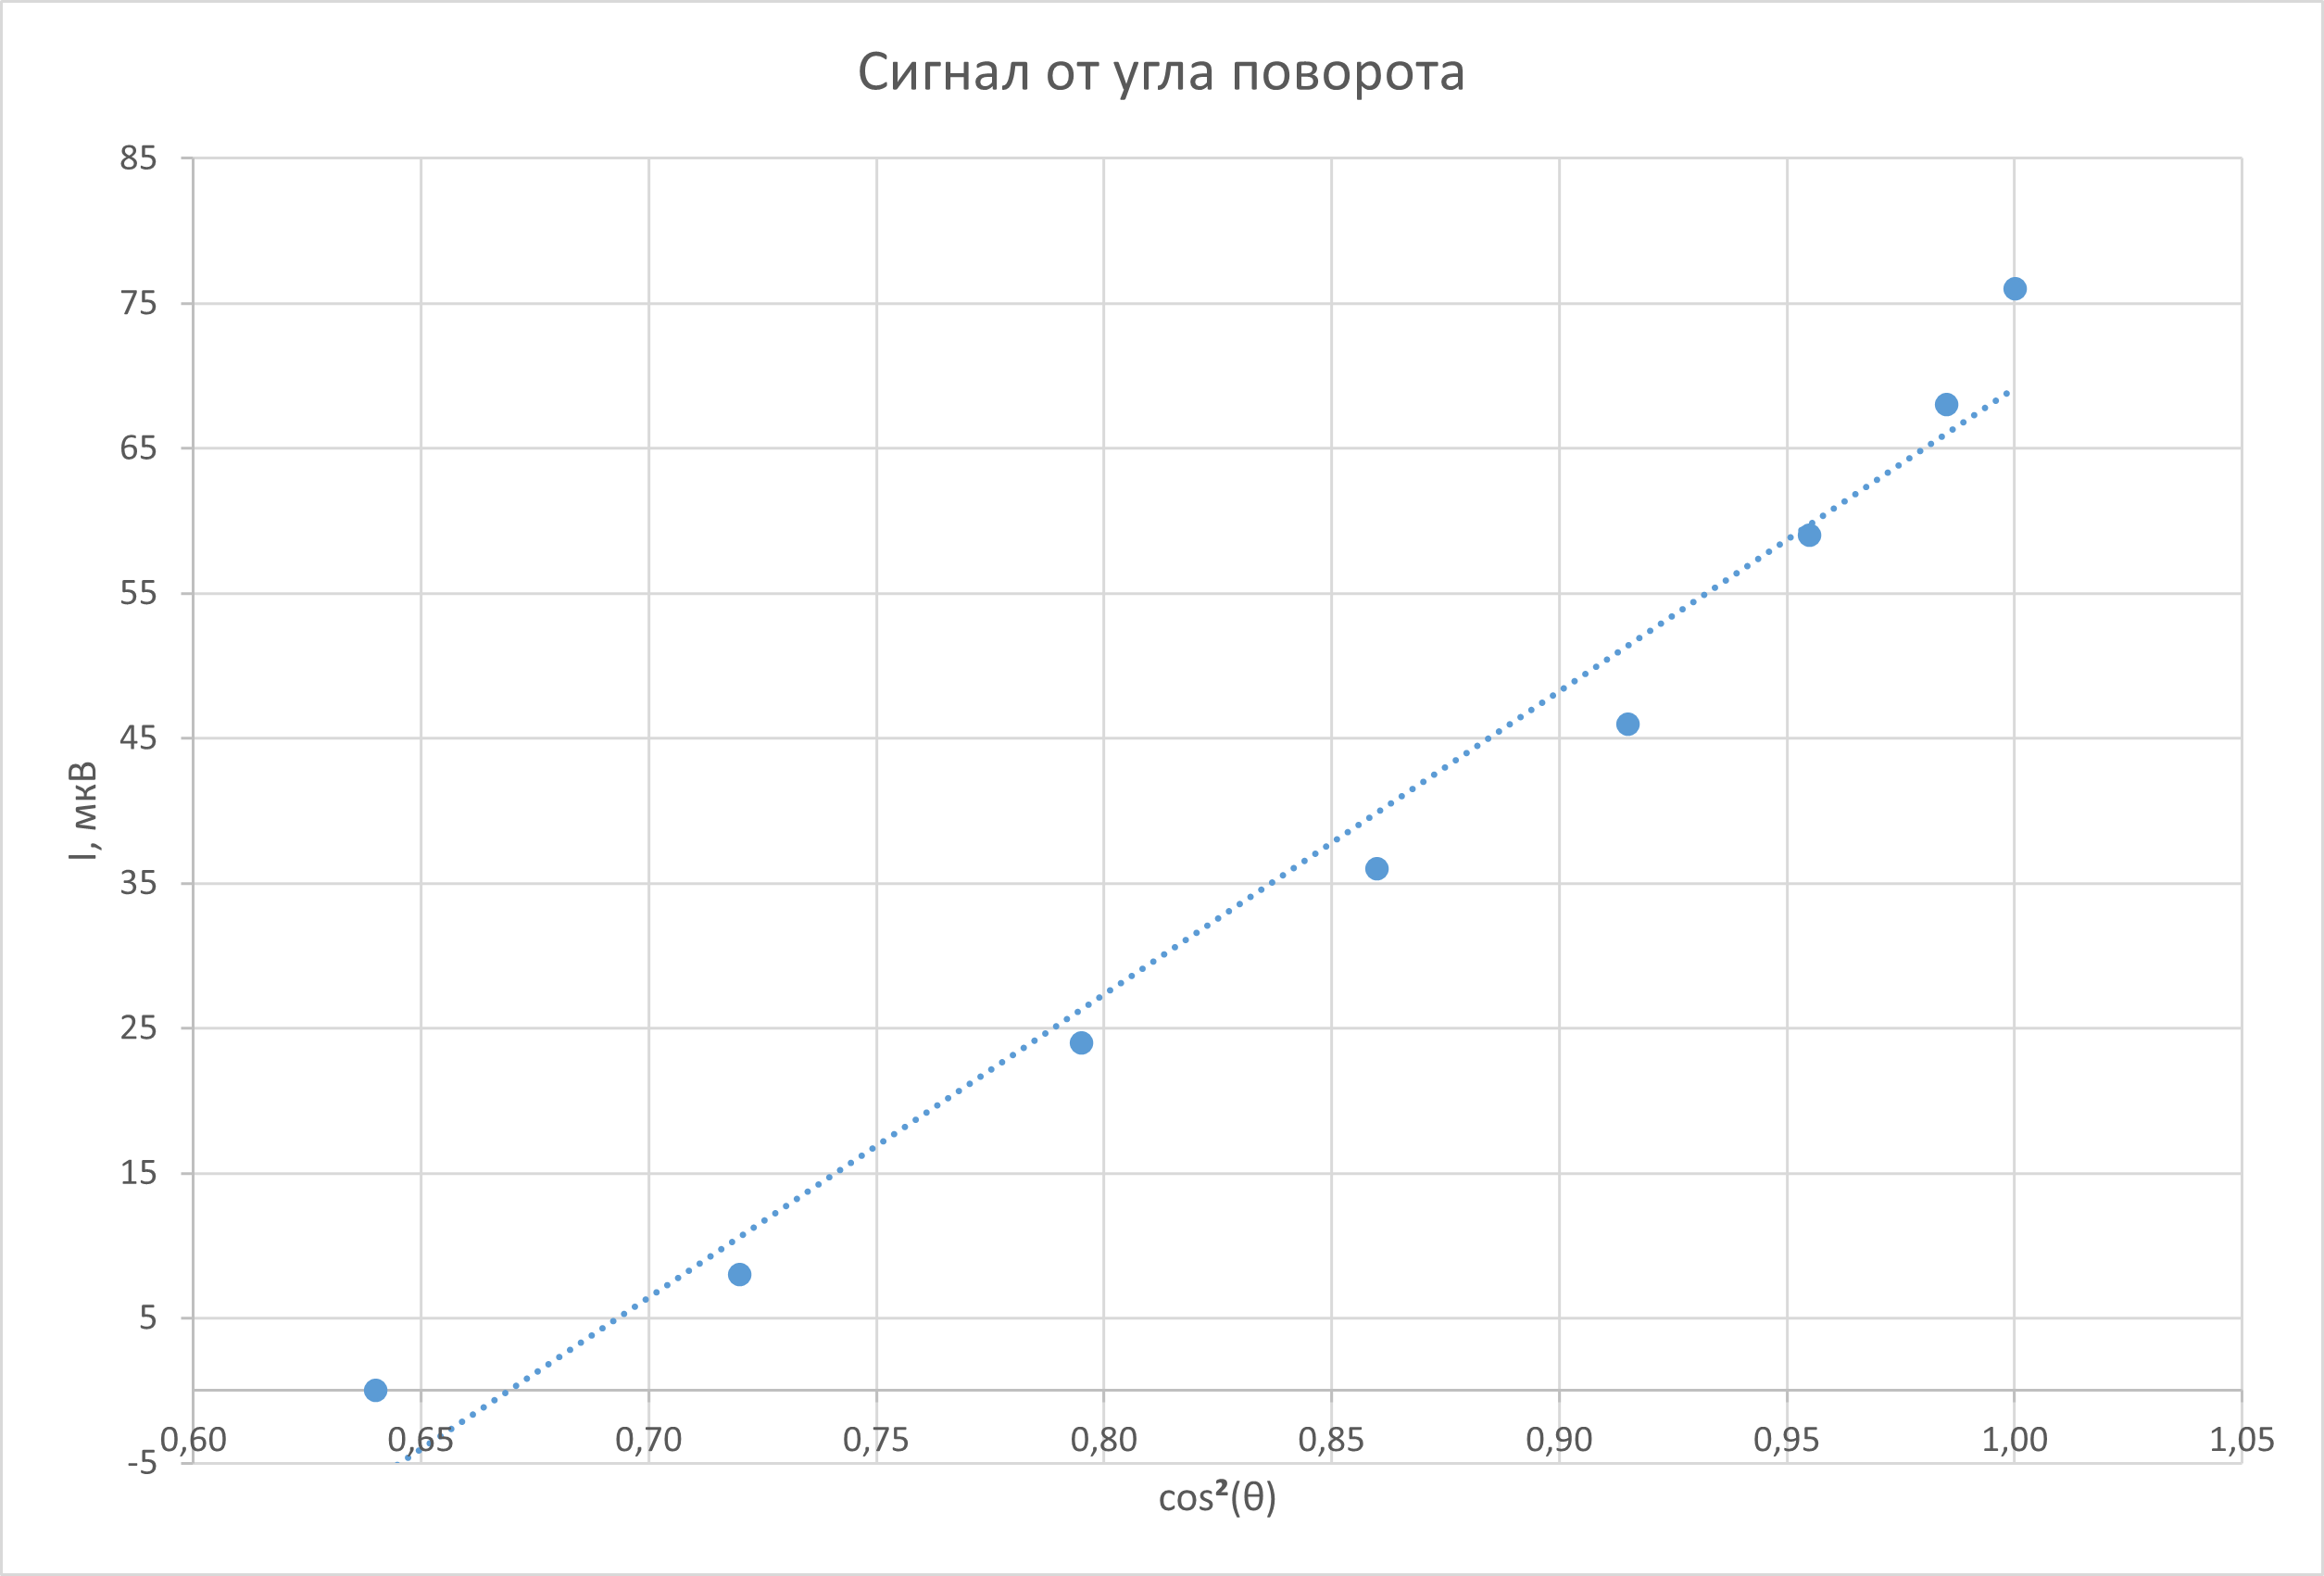
\includegraphics[scale=0.7]{pic/plot1.png}
    \caption{График зависимости интенсивности отраженной волны от угла падения}
    \label{graph1}
\end{figure}

\subsection{Интерференция волн, отражённых от зеркала и решётки}
\begin{figure}[H]
    \centering
    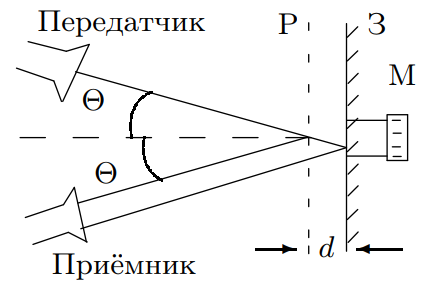
\includegraphics[scale=0.55]{pic/first_schema.png}
    \caption{Схема №1 с зеркалом и решёткой для наблюдения интерференции радиоволн}
    \label{fig:schema_1}
\end{figure}
Для исследования интерференции миллиметровых волн была собрана и отъюстирована на максимальный сигнал установка с рис. \ref{fig:schema_1}. Между приемником и излучателем была помещена металлическая решетка Р, частично пропускающая сигнал до зеркала З, в результате чего получались две компоненты излучения с разностью хода между ними, равной $\Delta = 2d\cos\theta$. 

Изменяя расстояние между зеркалом и решеткой при помощи микрометрического винта, мы измерили зависимость интенсивности принимаемого сигнала от координаты $x$ подвижного зеркала. Результаты представлены на графике \ref{fig:plot2} ниже и таблице \ref{tab2} в приложении. 

\begin{figure}[H]
    \centering
    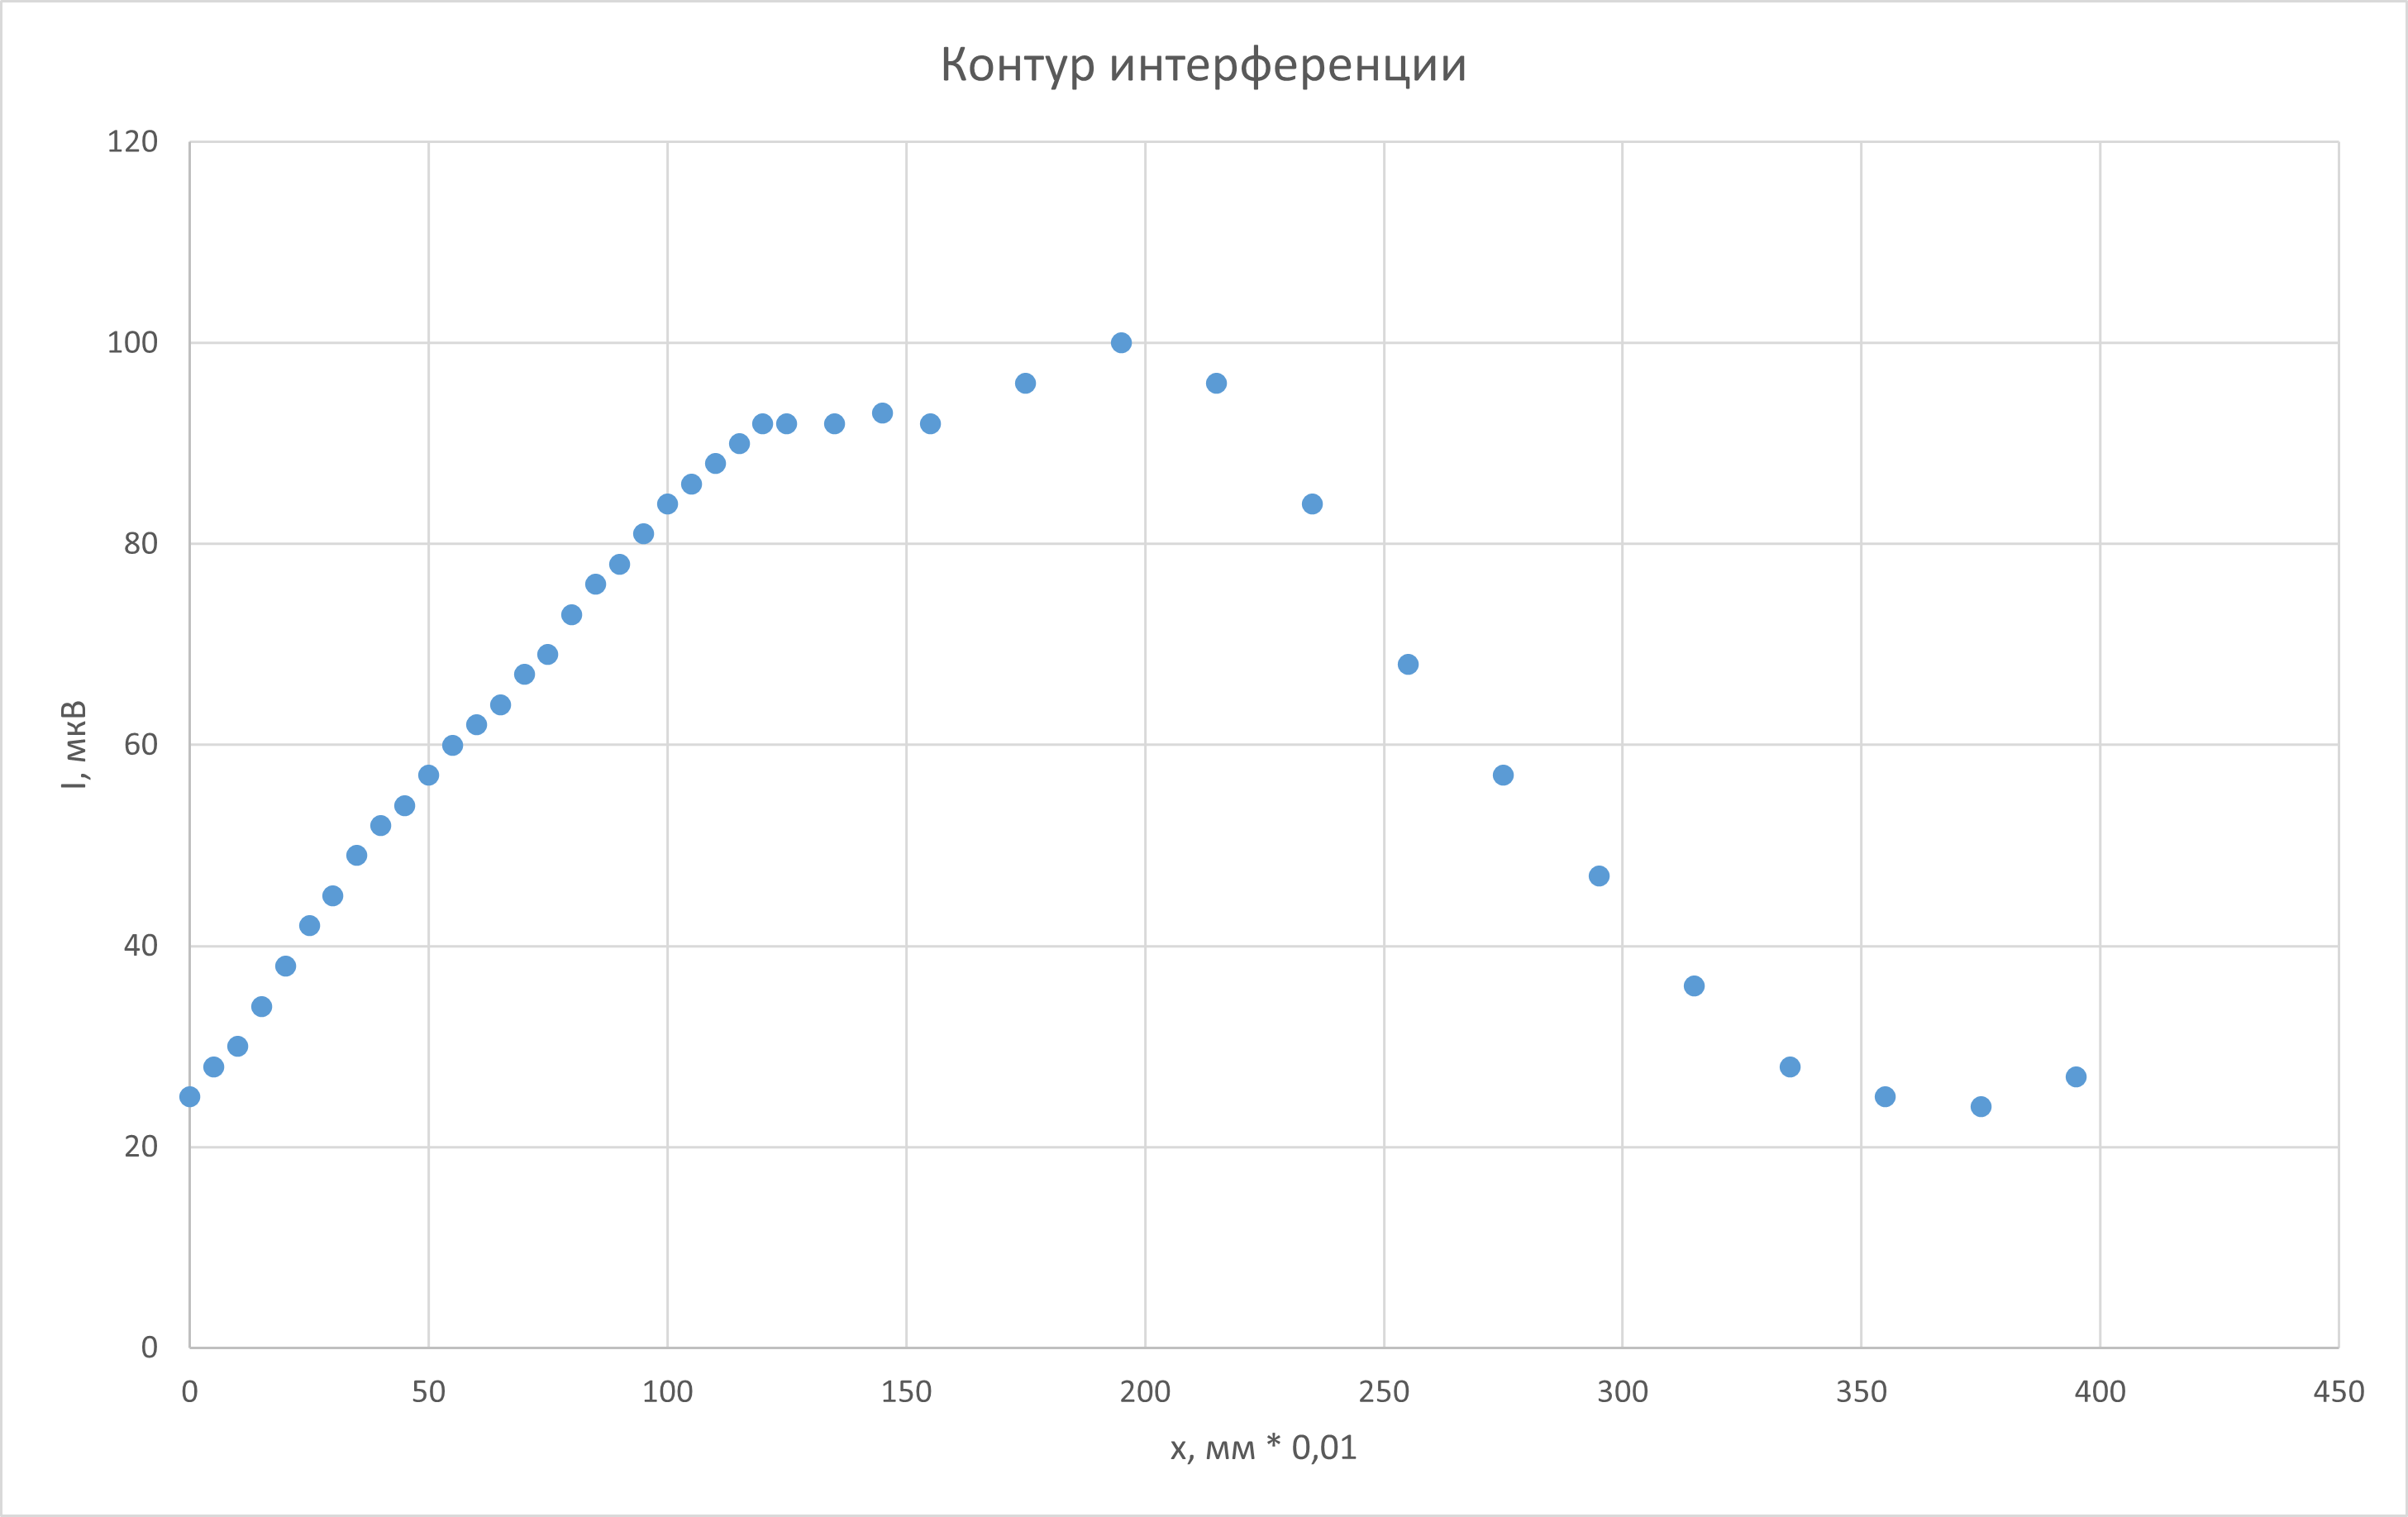
\includegraphics[scale=0.7]{pic/plot2.png}
    \caption{График зависимости интенсивности от расстояния между зеркалом и решёткой}
    \label{fig:plot2}
\end{figure}

По графику видно, что период изменения интенсивности равен $x=(4,3\pm0,2)$ мм, где погрешность определяется преимущественно погрешностью измерения длины. Отсюда с учётом $\theta\approx 0^\circ$ длина волны составляет $\lambda = (8,6 \pm 0,4)\text{ мм}$. При этом частота волн, генерируемых в установке соответствует длине волны $\lambda_{\text{gen}} \approx 8,3\text{ мм}$, что совпадает с полученным экспериментально значением в пределах одного стандартного отклонения.

\subsection{Интерферометр Майкельсона}
\begin{figure}[H]
    \centering
    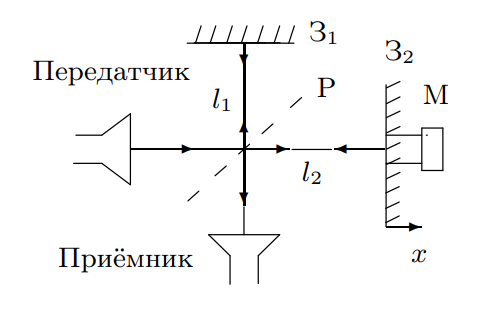
\includegraphics[scale=0.7]{pic/Michelson.png}
    \caption{Интерферометр Майкельсона}
    \label{fig:Michelson}
\end{figure}

В данной части работы использовалась установка, представленная на рис. \ref{fig:Michelson}~--- интерферометр Майкельсона. Изменение координаты отражающей подвижной пластинки приводит к изменению интерференционной картины и чередаванию максимумов и минимумов на приемнике. Снятая зависимость номера максимума от координаты представлена на графике \ref{fig:plot3} и в таблице \ref{tab3} приложения. 

\begin{figure}[H]
    \centering
    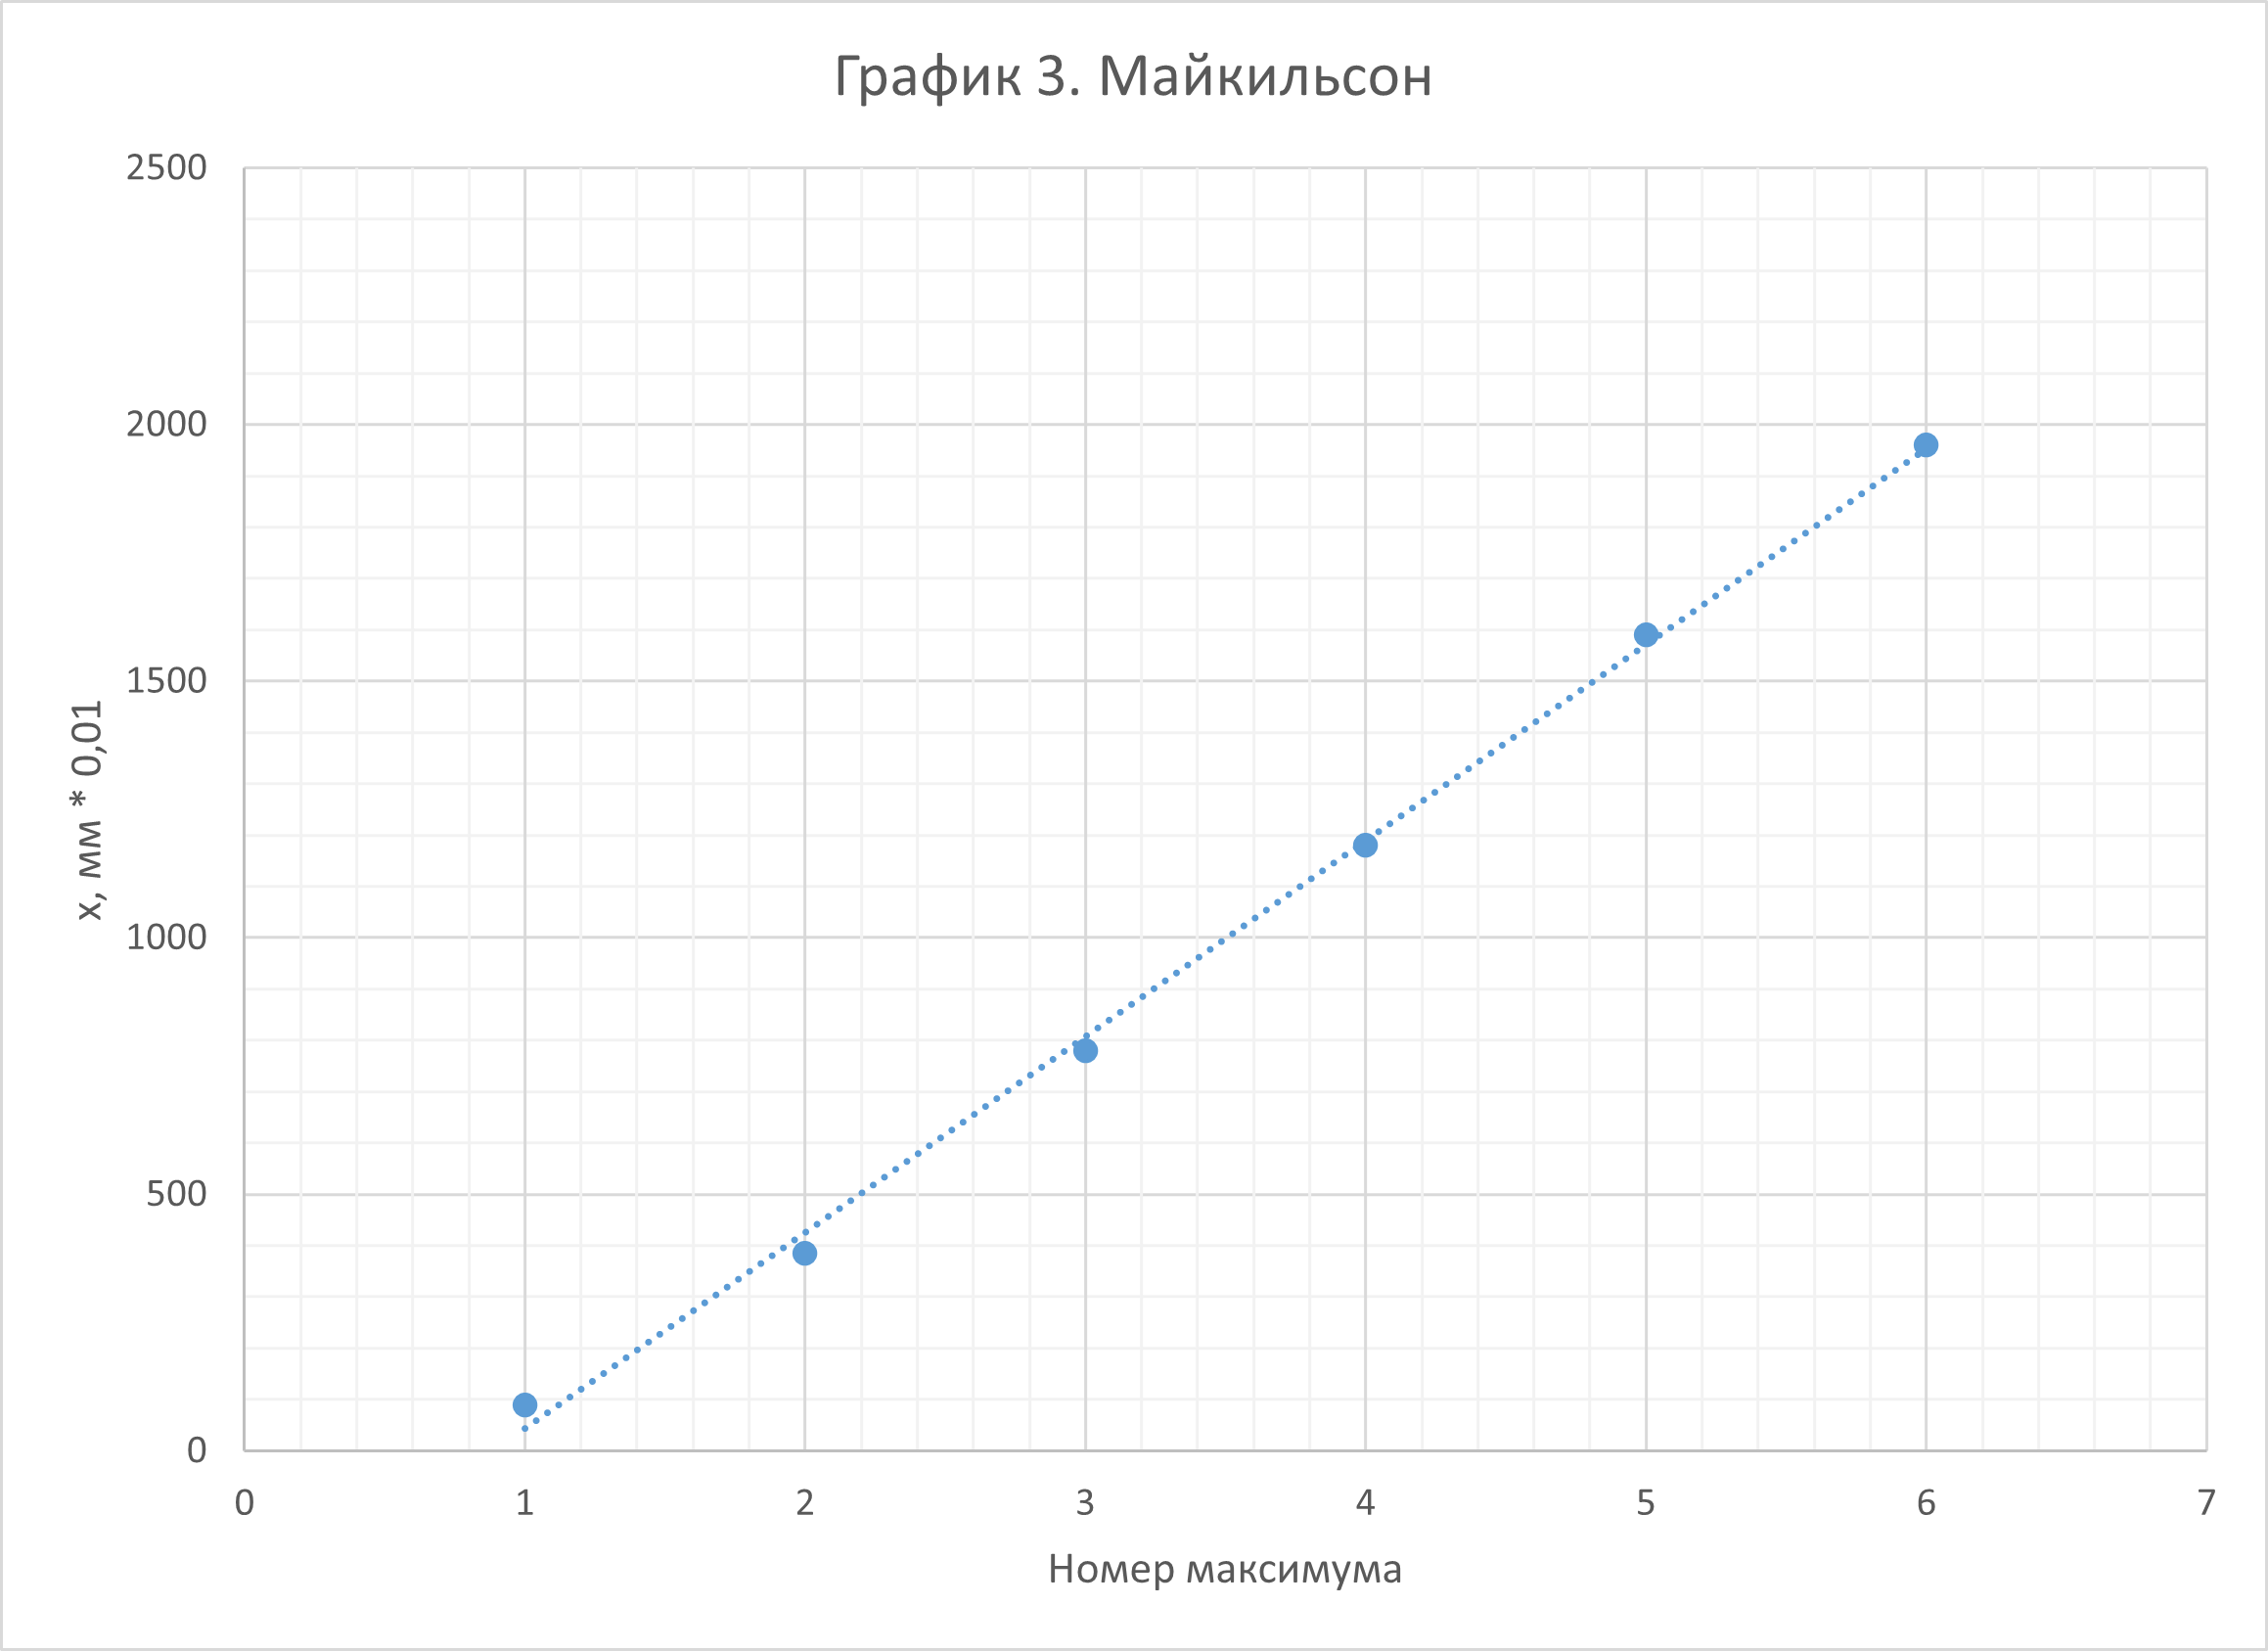
\includegraphics[scale=0.7]{pic/plot3.png}
    \caption{График зависимости координаты интерференционного максимума от его номера}
    \label{fig:plot3}
\end{figure}

Из графика по коэффициенту наклона определяется длина волны излучения: $\lambda_M = (7,6 \pm 0,4) \text{ мм}$. Погрешность определяется методом наименьших квадратов и погрешностью измерения длины.

\subsubsection{Определение показателя преломления пластинки}
Поместив в точке интерференционного максимума перед подвижным зеркалом пластинку из диэлектрика, мы наблюдали уменьшение напряжения на вольтметре, что свидетельствует об изменении разности хода лучей. Компенсируя его смещением отражающей пластинки, мы измерили добавочную разность хода: $\Delta = (1,13 \pm 0,02)\text{ мм}$. Данное значение было измерено по графику \ref{fig:plot4} как смещение интерференционного максимума относительно начала измерений.

\begin{figure}[H]
    \centering
    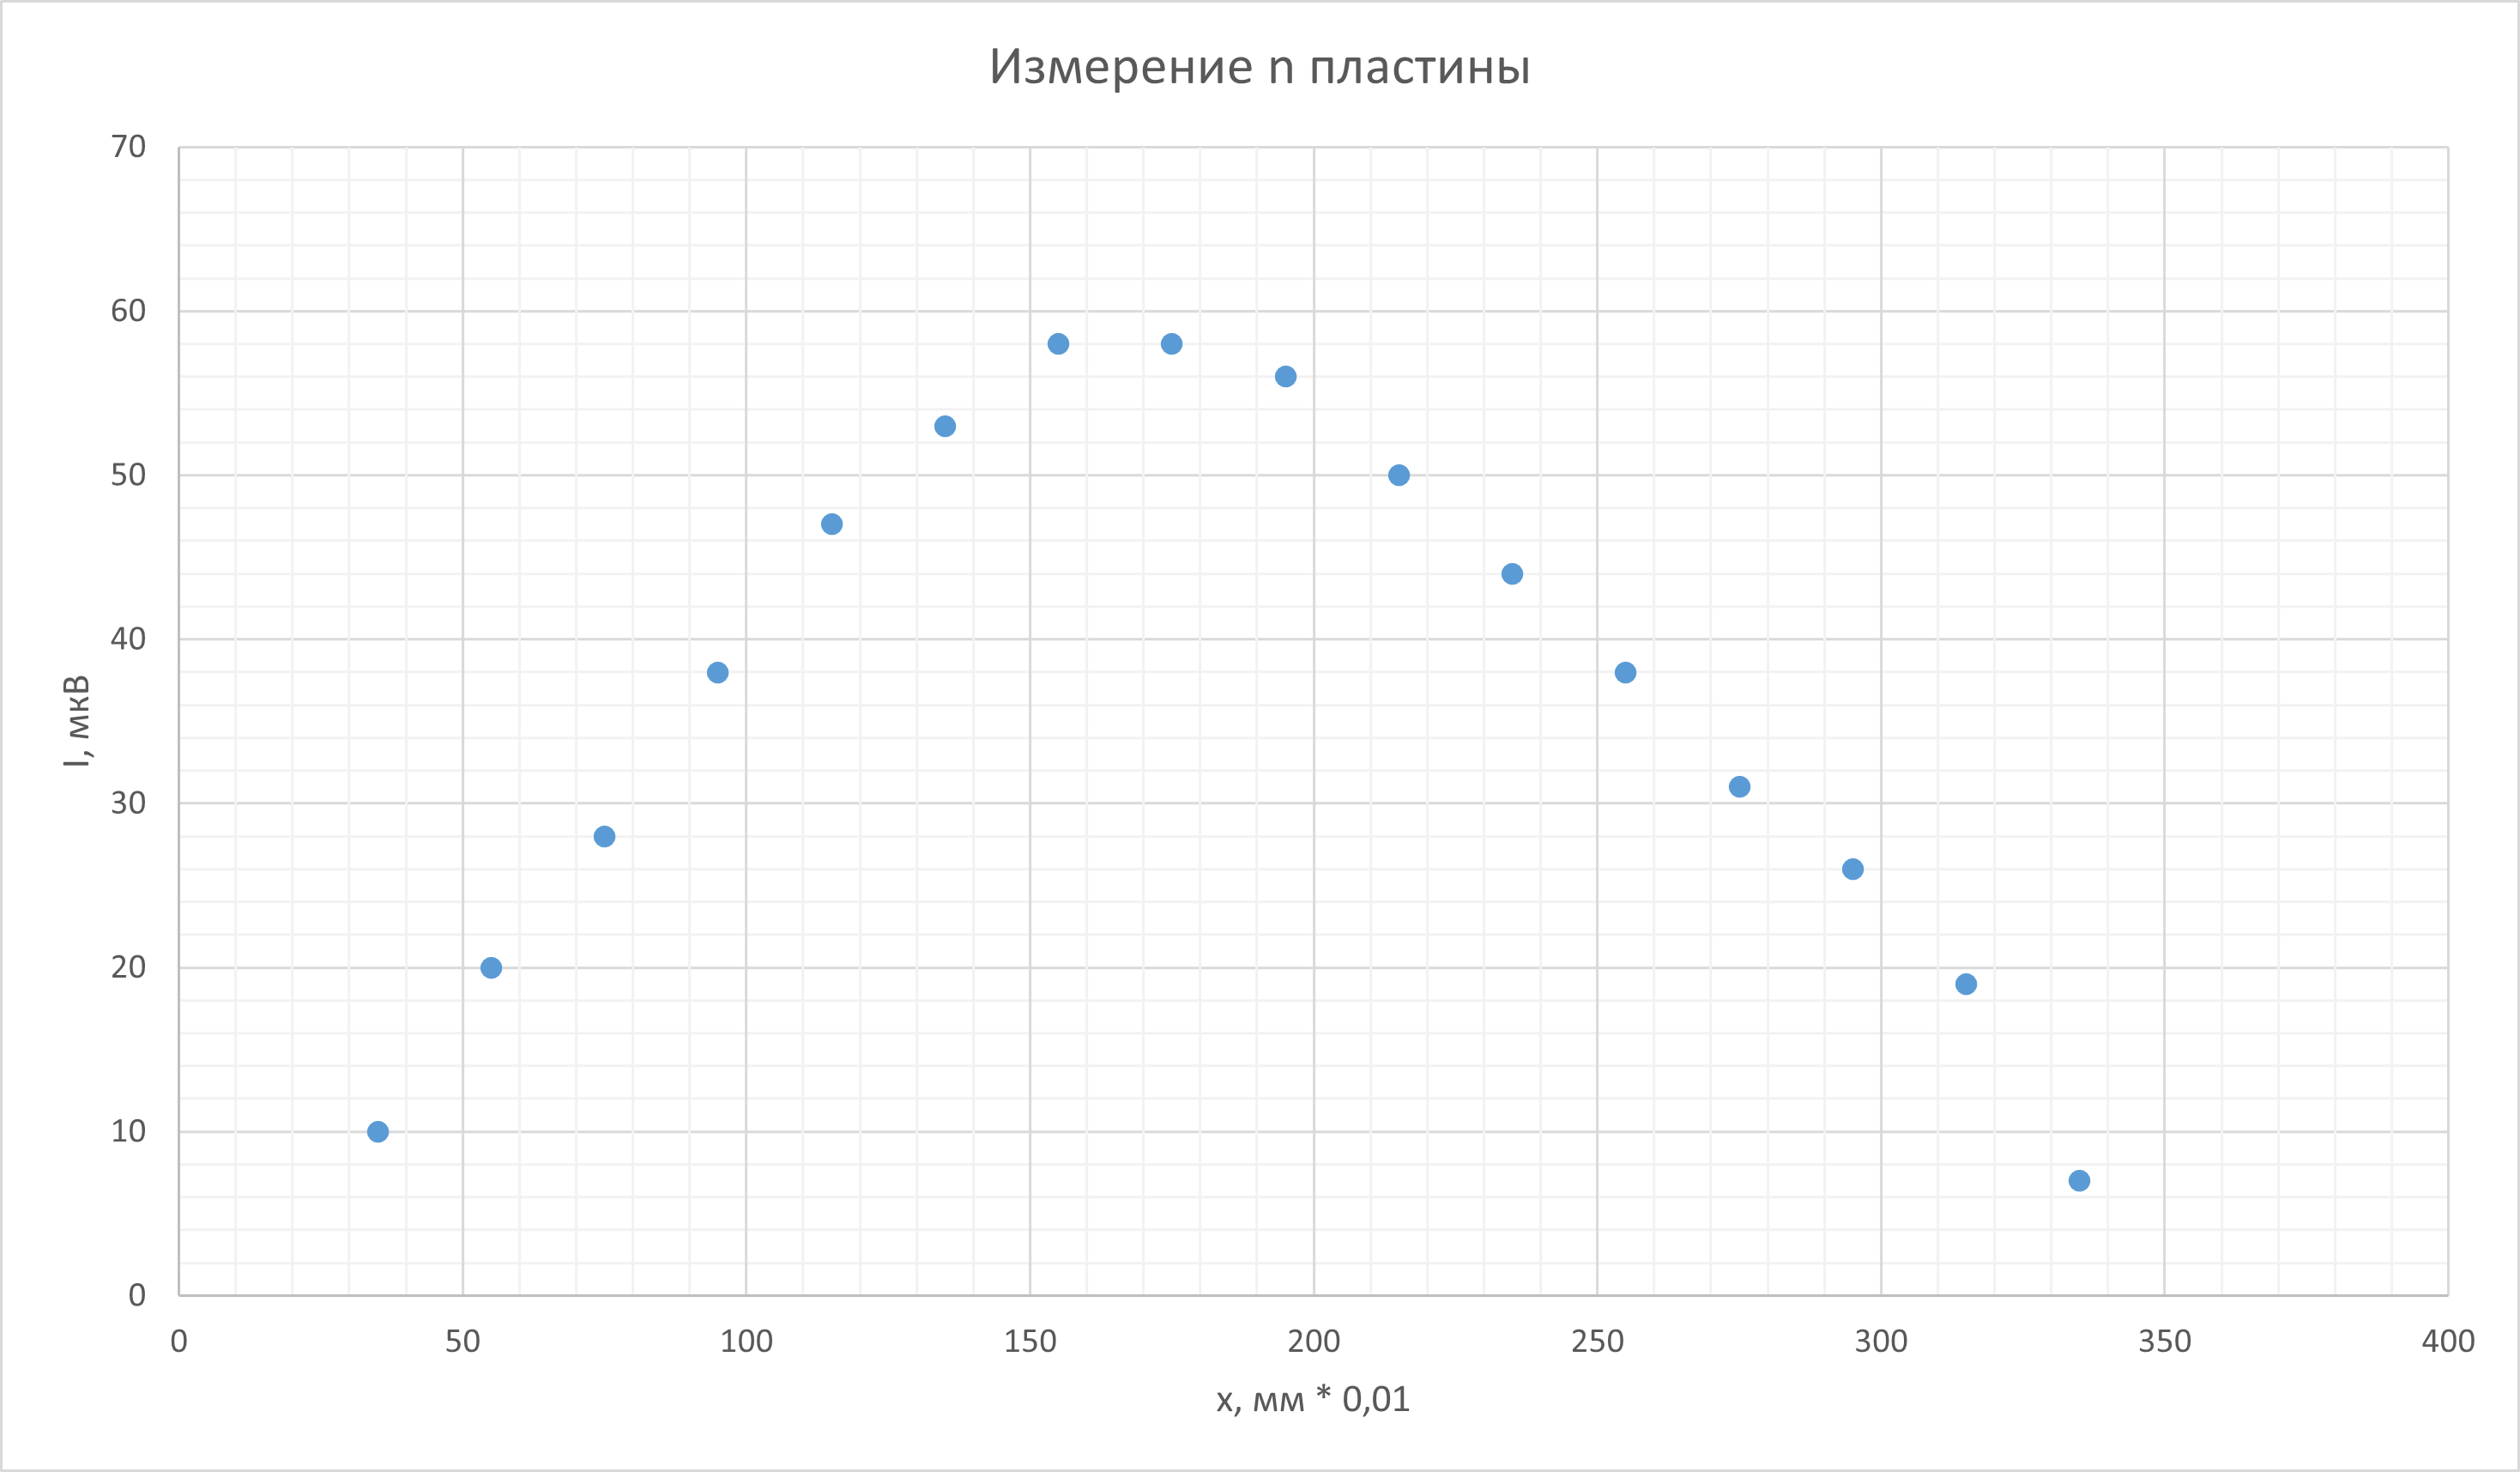
\includegraphics[scale=0.7]{pic/plot4.png}
    \caption{График зависимости зависимости интенсивности от смещения зеркала при добавлении диэлектрика}
    \label{fig:plot4}
\end{figure}

Используя формулу $\Delta = h(n-1)$, где толщина пластинки $h = 3,25\text{ мм}$ (здесь старый ход лучей~--- $l_0+h$, новый~---$l_0 + nh$), получаем показатель преломления материала пластинки: $n = 1,34 \pm 0,03$.
Табличное значение~--- $n_{\text{tab}} = 1,34$~--- совпадает с измеренным в пределах погрешности. 

\section{Выводы}
При помощи оптических схем можно изучать радиоволны СВЧ-диапазона. При с достаточно высокой точностью можно определить такие параметры излучения, как длина волны. При помощи интерферометра Майкельсона можно также определить показатель преломления пластинки из диэлектрического материала. 

\newpage

\section{Приложение}
\begin{table}[H]
    \centering
    \begin{tabular}{|l|l|l|l|}
    \hline
        x, мм $\cdot 10^{-2}$ & U, мВ & x, мм$\cdot 10^{-2}$ & U, мВ \\ \hline
        0 & 25 & 100 & 84 \\ \hline
        5 & 28 & 105 & 86 \\ \hline
        10 & 30 & 110 & 88 \\ \hline
        15 & 34 & 115 & 90 \\ \hline
        20 & 38 & 120 & 92 \\ \hline
        25 & 42 & 125 & 92 \\ \hline
        30 & 45 & 135 & 92 \\ \hline
        35 & 49 & 145 & 93 \\ \hline
        40 & 52 & 155 & 92 \\ \hline
        45 & 54 & 175 & 96 \\ \hline
        50 & 57 & 195 & 100 \\ \hline
        55 & 60 & 215 & 96 \\ \hline
        60 & 62 & 235 & 84 \\ \hline
        65 & 64 & 255 & 68 \\ \hline
        70 & 67 & 275 & 57 \\ \hline
        75 & 69 & 295 & 47 \\ \hline
        80 & 73 & 315 & 36 \\ \hline
        85 & 76 & 335 & 28 \\ \hline
        90 & 78 & 355 & 25 \\ \hline
        95 & 81 & 375 & 24 \\ \hline
        100 & 84 & 395 & 27 \\ \hline
    \end{tabular}
    \caption{Зависимость интенсивности от расстояния между зеркалом и решёткой}
    \label{tab2}
\end{table}

\begin{table}[H]
    \centering
    \begin{tabular}{|l|l|}
    \hline
        № & x, мм $\cdot 10^{-2}$ \\ \hline
        1 & 90 \\ \hline
        2 & 385 \\ \hline
        3 & 780 \\ \hline
        4 & 1180 \\ \hline
        5 & 1590 \\ \hline
        6 & 1960 \\ \hline
    \end{tabular}
    \caption{Зависимость координаты интерференционного максимума от его номера}
    \label{tab3}
\end{table}